加载了网络之后,Cytoscape的界面如图~\ref{fig:2.1}~所示。

\begin{figure}[!h]
\centering
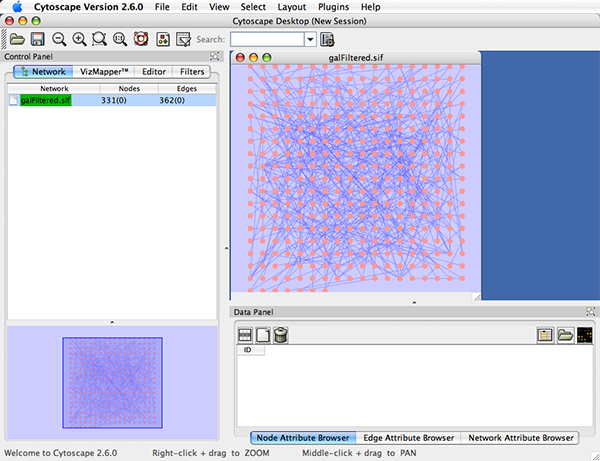
\includegraphics[width=\textwidth]{images/cytoscape_startup_network_26.png}
\caption{Cytoscape加载网络后的界面截图}
\label{fig:2.1}
\end{figure}

主界面由多个组件构成,包括:
\begin{itemize}
\item 顶部的菜单(稍后会对各个菜单做详细介绍)。
\item 工具栏,包含了各种常用功能。从菜单中也能使用这些功能。鼠标指针在这些图标上停留片刻就能看到有关的提示。
\item 网络管理面板(左上方的面板)。其中有可关闭的网络全局浏览面板(左下方)。
\item 网络查看主窗口,网络就显示在这个窗口中。
\item 属性浏览器面板(底部的面板),显示所选择的节点和边的属性。在这个面板中还可以对这些属性的值进行修改。
\end{itemize}

网络管理和属性浏览器面板是可以拖拽的标签面板,被称为~CytoPanels~。通过点击~CytoPanel~右上角的浮动窗口(Float Window)控件~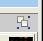
\includegraphics{images/float_icon.png}~可以将这些面板设为浮动状态。

如果选择了这个控件,例如属性浏览器面板上的这个控件,就会出现两个~Cytoscape~的窗口,一个是主窗口,另一个是名为CytoPanel 2的新窗口,如下图所示。当鼠标指针指向单元格时,会看到弹出信息。

{\centering
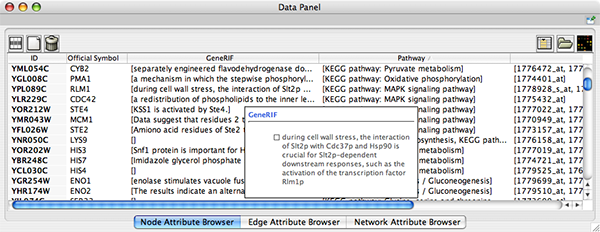
\includegraphics[width=\textwidth]{images/attribute_browser_26.png}
}

在图中可以看到,CytoPanel 2~现在有一个~Dock Window~控件。如果点选这个控件,这个窗口就会回到主窗口中。


